% Provenance (never printed): old premiere S material on the lithosphere and the
% asthenosphere (chemical and mechanical layers, the low-velocity zone, the
% geotherm, isostasy); see sources/book2/PROVENANCE.md. S speeds from
% figdata/grade-11/prem_profiles.py (part upper), the geotherm and the solidus
% from geotherm_solidus.py, the elevations from hypsometry.py (ETOPO1).
% Glacial rebound belongs to g12; lithostatic pressure (term) to g12.
\chapter{Lithosphère et asthénosphère}\label{ch:g11:lithosphere-asthenosphere}

Les neuf dixièmes d'un iceberg se trouvent sous l'eau~: la glace flotte
parce qu'elle est un peu moins dense que la mer, et elle s'enfonce dans
l'eau jusqu'à ce que l'eau qu'elle déplace pèse autant que l'iceberg tout
entier. Les chaînes de montagnes se comportent à peu près de la même façon.
Sous les plus hautes, la croûte est près de deux fois plus épaisse que
d'habitude, et la plus grande partie de ce surplus de croûte est cachée
en dessous, comme la glace sous la ligne de flottaison. Mais un iceberg
flotte dans un liquide, et le manteau situé sous une chaîne de montagnes est
de la roche solide. Ce chapitre montre comment un solide peut se comporter
comme un fluide sur lequel flotte l'enveloppe externe de la Terre, et ce
qu'est cette enveloppe.
% ledger: usgs:ice-density, karplus:tibet-moho, cm95:crust

\begin{recall}
La Terre comprend une croûte, un manteau et un noyau (livre~1, année~6). Le
\omterm{def:g11:seismic-structure:moho}{Moho}, à la base de la croûte, se trouve en moyenne à environ \qty{41}{km} de
profondeur sous les continents et à quelques kilomètres sous le fond des
océans~; les vitesses sismiques et les masses volumiques sont connues à
chaque profondeur grâce à un \omterm{def:g11:seismic-structure:reference-model}{modèle de Terre de référence}
(\cref{ch:g11:seismic-structure}). La roche est de plus en plus chaude avec
la profondeur, d'environ 25 à \qty{30}{\celsius} par kilomètre près de la
surface (livre~1, année~6). Un corps qui flotte dans un liquide déplace un
poids de liquide égal à son propre poids, et la pression à la base d'une
colonne de matière est le poids de la colonne divisé par sa surface (les
livres de physique).
\end{recall}
% ledger: cm95:crust, usgs:crust-thickness, usgs:gradient-29 (Book 1 rows)

\begin{omfigure}
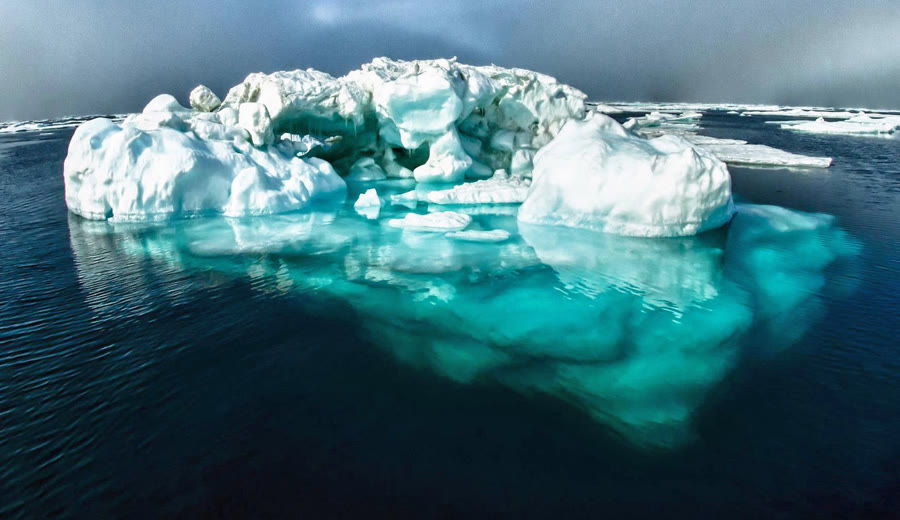
\includegraphics[width=0.66\linewidth]{images/book2/g11-noaa-iceberg.jpg}

{\small Un iceberg vu juste au-dessus de l'eau~: la glace située sous la
surface, qui transparaît à travers la mer limpide, est bien plus grande que
la partie émergée. Photographie~: NOAA (domaine public).}
\end{omfigure}
% ledger: photo:g11-iceberg

\section{Deux façons de découper la Terre en couches}

La croûte, le manteau et le noyau sont des couches de \emph{matériaux}
différents~: la croûte est faite de roches riches en silicium, en aluminium
et en oxygène, le manteau d'une roche plus dense, le noyau de métal. Mais la
partie externe de la Terre peut aussi être découpée selon la façon dont sa
roche se \emph{comporte} quand des forces agissent sur elle pendant très
longtemps.

\begin{definition}[Lithosphère~; asthénosphère]\label{def:g11:lithosphere-asthenosphere:lithosphere}
La \emph{lithosphère}\index{lithosphere@lithosphère} est l'enveloppe externe
rigide de la Terre~: la croûte et la partie la plus haute et la plus froide
du manteau, qui, ensemble, se découpent en plaques tectoniques et ne
s'écoulent pas. L'\emph{asthénosphère}\index{asthenosphere@asthénosphère}
est la couche du manteau située sous la lithosphère, plus chaude et moins
résistante, qui s'écoule lentement sur de longues durées, comme une pâte
très ferme.
\end{definition}

La limite entre les deux se trouve à environ 70 à \qty{100}{km} de
profondeur sous les océans et sous la plupart des continents, et plus bas
sous les parties les plus anciennes des continents~; à travers les
États-Unis, par exemple, l'épaisseur de la \omterm{def:g11:lithosphere-asthenosphere:lithosphere}{lithosphère} va d'environ
\qty{40}{km} à l'ouest à plus de \qty{200}{km} au milieu du continent. La
base de la \omterm{def:g11:lithosphere-asthenosphere:lithosphere}{lithosphère} n'est pas le \omterm{def:g11:seismic-structure:moho}{Moho}~: la \omterm{def:g11:lithosphere-asthenosphere:lithosphere}{lithosphère} est surtout faite
de roche du manteau.
% ledger: rs09:lab, fischer:lab, porter:lab, usgs:lithosphere-80km (Book 1 row)

\begin{omfigure}
\begin{tikzpicture}[x=1cm, y=-0.0125cm, font=\footnotesize]
% depths to scale: crust 41 km (cm95:crust), lithosphere 100 km (rs09:lab), 0-400 km
  \shade[top color=omLithPeridotite!70, bottom color=omLithPeridotite!25] (5,100) rectangle (8,400);
  \fill[omLithGranite!55] (0,0) rectangle (3,41);
  \fill[omLithPeridotite!55] (0,41) rectangle (3,400);
  \fill[black!25] (5,0) rectangle (8,100);
  \draw (0,0) rectangle (3,400);
  \draw (5,0) -- (5,400) (8,0) -- (8,400) (5,0) -- (8,0);
  \draw[line width=0.8pt] (0,41) -- (3,41);
  \draw[line width=0.8pt, densely dashed] (5,100) -- (8,100);
  \draw[densely dotted, black!60] (3,41) -- (5,41);
  \node at (1.5,20) {croûte};
  \node[align=center] at (1.5,220) {manteau};
  \node[align=center] at (6.5,50) {lithosphère\\rigide};
  \node[align=center] at (6.5,180) {asthénosphère\\peu résistante,\\s'écoule lentement};
  \node[align=center, text=black!70] at (6.5,340) {manteau profond};
  \node[anchor=south, font=\small] at (1.5,0) {par matériau};
  \node[anchor=south, font=\small] at (6.5,0) {par comportement};
  \foreach \d in {0,100,200,300,400} {\draw (-0.1,\d) -- (0,\d); \node[anchor=east] at (-0.1,\d) {\d};}
  \node[anchor=east, rotate=90, anchor=south] at (-0.9,200) {profondeur (\unit{km})};
  \node[anchor=south, font=\scriptsize, align=center] at (4,41) {Moho\\(\qty{41}{km})};
  \node[anchor=west, align=left] at (8.15,100) {base de la\\lithosphère\\(environ \qty{100}{km})};
\end{tikzpicture}

{\small Les \qty{400}{km} supérieurs de la Terre sous un continent, à
l'échelle. À gauche~: les couches par matériau. À droite~: les couches par
comportement. La \omterm{def:g11:lithosphere-asthenosphere:lithosphere}{lithosphère} rigide contient toute la croûte et le sommet du
manteau~; l'\omterm{def:g11:lithosphere-asthenosphere:lithosphere}{asthénosphère} n'a pas de limite inférieure nette.}
\end{omfigure}

\section{La zone à faible vitesse}

Les ondes sismiques révèlent l'\omterm{def:g11:lithosphere-asthenosphere:lithosphere}{asthénosphère}. Presque partout dans la Terre,
les vitesses sismiques augmentent avec la profondeur, parce que la roche est
de plus en plus comprimée. Sous la \omterm{def:g11:lithosphere-asthenosphere:lithosphere}{lithosphère}, c'est l'inverse qui se
produit.

\begin{definition}[Zone à faible vitesse]\label{def:g11:lithosphere-asthenosphere:lvz}
La \emph{zone à faible vitesse}\index{zone a faible vitesse@zone à faible vitesse}
est la couche du manteau supérieur, sous la \omterm{def:g11:lithosphere-asthenosphere:lithosphere}{lithosphère}, dans
laquelle les ondes sismiques se propagent plus lentement que dans la roche
située au-dessus et au-dessous.
\end{definition}

Dans le \omterm{def:g11:seismic-structure:reference-model}{modèle de Terre de référence}, la vitesse des \omterm{def:g11:seismic-structure:body-waves}{ondes S} diminue
lentement du \omterm{def:g11:seismic-structure:moho}{Moho} jusqu'à \qty{220}{km}, puis remonte d'un coup. Partout dans
le monde, les études sismiques trouvent une chute brutale de la vitesse
quelque part entre 70 et \qty{100}{km}~: le sommet de l'\omterm{def:g11:lithosphere-asthenosphere:lithosphere}{asthénosphère}. La
roche y est assez chaude pour être proche de la fusion, et elle peut
contenir un tout petit peu de liquide~; elle peut aussi renfermer plus d'eau
que la roche située au-dessus. Une roche proche de la fusion est peu
résistante~: elle ralentit les ondes sismiques, et elle peut s'écouler.
% ledger: data:prem, rs09:lab, fischer:lab, porter:lab

\begin{omfigure}
\begin{tikzpicture}
\begin{axis}[omrecord, omdepth, width=0.6\linewidth, height=6.0cm, xmin=3.0, xmax=5.0, ymin=0, ymax=400,
  xlabel={vitesse des ondes S (\unit{km/s})}, ylabel={profondeur (\unit{km})}, xtick={3.0,3.5,...,5.0},
  xticklabel style={/pgf/number format/fixed, /pgf/number format/precision=1},
  tick label style={font=\small}, label style={font=\small}]
% computed in figdata/grade-11/prem_profiles.py (part upper); ledger: data:prem
\fill[black!10] (axis cs:3.0,80) rectangle (axis cs:5.0,220);
\addplot[omProp, line width=0.9pt] table[x=vs, y=depth] {figdata/out/grade-11-prem_profiles-upper.dat};
\node[font=\scriptsize, anchor=west, align=left] at (axis cs:3.1,150) {zone à\\faible vitesse};
\node[font=\scriptsize, anchor=west] at (axis cs:3.95,12) {croûte};
\end{axis}
\end{tikzpicture}

{\small La vitesse des \omterm{def:g11:seismic-structure:body-waves}{ondes S} dans les \qty{400}{km} supérieurs du \omterm{def:g11:seismic-structure:reference-model}{modèle de
Terre de référence}. Sous la croûte, la vitesse diminue lentement avec la
profondeur jusqu'à \qty{220}{km} (en grisé à partir de \qty{80}{km}), puis
augmente de nouveau par sauts brusques.}
\end{omfigure}

\section{Le géotherme}

\begin{definition}[Géotherme~; gradient géothermique]\label{def:g11:lithosphere-asthenosphere:geotherm}
Un \emph{géotherme}\index{geotherme@géotherme} est la courbe de la
température en fonction de la profondeur sous un lieu. Le \emph{gradient
géothermique}\index{gradient geothermique@gradient géothermique} est
l'augmentation de la température par unité de profondeur, en degrés par
kilomètre.
\end{definition}

Les forages ne mesurent le \omterm{def:g11:lithosphere-asthenosphere:geotherm}{géotherme} que dans les premiers kilomètres, où la
température augmente de 25 à \qty{30}{\celsius} par kilomètre (livre~1,
année~6). Plus bas, on le calcule à partir de la chaleur qui s'échappe par la
surface et des propriétés des roches~; le \cref{ch:g12:internal-heat} montre
d'où vient cette chaleur. Deux faits façonnent le résultat. Une partie de la
chaleur est produite à l'intérieur même de la croûte supérieure~: le
gradient est donc le plus fort près de la surface et plus faible sous la
croûte. Et dans l'\omterm{def:g11:lithosphere-asthenosphere:lithosphere}{asthénosphère}, qui s'écoule, le lent mouvement de la roche
transporte la chaleur et égalise la température~: elle n'augmente que
d'environ \qty{0.45}{\celsius} par kilomètre. On place la base de la
\omterm{def:g11:lithosphere-asthenosphere:lithosphere}{lithosphère} là où le \omterm{def:g11:lithosphere-asthenosphere:geotherm}{géotherme} pentu de la \omterm{def:g11:lithosphere-asthenosphere:lithosphere}{lithosphère} rejoint celui, peu
pentu, de l'\omterm{def:g11:lithosphere-asthenosphere:lithosphere}{asthénosphère}, vers \qty{1300}{\celsius}.
% ledger: usgs:gradient-29 (Book 1 row), b2dd10:continents, b2roy:provinces, roy:conductivity,
% katsura10:adiabat, porter:lab

\begin{omfigure}
\begin{tikzpicture}
\begin{axis}[omrecord, omdepth, width=0.7\linewidth, height=6.4cm, xmin=0, xmax=2000, ymin=0, ymax=300,
  xlabel={température (\unit{\celsius})}, ylabel={profondeur (\unit{km})}, xtick={0,500,...,2000},
  tick label style={font=\small}, label style={font=\small}]
% computed in figdata/grade-11/geotherm_solidus.py; ledger: b2dd10:continents, b2roy:provinces,
% roy:conductivity, porter:lab, katsura10:adiabat, hirschmann:solidus, data:prem
\fill[black!8] (axis cs:0,99.7) rectangle (axis cs:2000,300);
\addplot[omDef, line width=1.0pt] table[x=t_geotherm, y=depth_km] {figdata/out/grade-11-geotherm_solidus-geotherm.dat};
\addplot[omDef, densely dashed, restrict y to domain=99:300] table[x=t_cond, y=depth_km] {figdata/out/grade-11-geotherm_solidus-geotherm.dat};
\addplot[omProp, line width=1.0pt] table[x=t_solidus, y=depth_km] {figdata/out/grade-11-geotherm_solidus-geotherm.dat};
\draw[black!60] (axis cs:0,99.7) -- (axis cs:2000,99.7);
\node[font=\scriptsize, anchor=south west] at (axis cs:20,99.7) {base de la lithosphère};
\node[font=\scriptsize, anchor=north west] at (axis cs:20,102) {asthénosphère};
\node[font=\scriptsize, text=omDef, anchor=north west] at (axis cs:480,6) {géotherme};
\node[font=\scriptsize, text=omProp, anchor=west] at (axis cs:1300,22) {début de la fusion};
\end{axis}
\end{tikzpicture}

{\small Un \omterm{def:g11:lithosphere-asthenosphere:geotherm}{géotherme} modèle sous un continent (en bleu) et la température à
laquelle la roche du manteau (la péridotite, sans eau) commence à fondre (en
orange). Le \omterm{def:g11:lithosphere-asthenosphere:geotherm}{géotherme} est calculé à partir du flux de chaleur moyen des
continents et de propriétés mesurées des roches~; dans l'\omterm{def:g11:lithosphere-asthenosphere:lithosphere}{asthénosphère} (en
gris), il augmente lentement. Les tirets montrent comment se poursuivrait
l'augmentation plus forte de la \omterm{def:g11:lithosphere-asthenosphere:lithosphere}{lithosphère}. Les deux courbes sont le plus
proches, à environ \qty{140}{\celsius} l'une de l'autre, près de la base de
la \omterm{def:g11:lithosphere-asthenosphere:lithosphere}{lithosphère}.}
\end{omfigure}
% values: lab_km 99.7, t_lab_c 1345, closest_gap_c 144 (figdata/grade-11/geotherm_solidus.py)

La température de fusion de la roche du manteau augmente avec la
profondeur, parce que la roche est de plus en plus comprimée (livre~1,
année~6)~: environ \qty{1120}{\celsius} en surface, près de
\qty{1500}{\celsius} à \qty{100}{km}. Dans le modèle, le \omterm{def:g11:lithosphere-asthenosphere:geotherm}{géotherme} s'en
approche le plus juste sous la \omterm{def:g11:lithosphere-asthenosphere:lithosphere}{lithosphère}, à environ \qty{140}{\celsius}
en dessous. Un peu d'eau, ou un manteau un peu plus chaud, comble l'écart~:
dans l'ouest des États-Unis, où la \omterm{def:g11:lithosphere-asthenosphere:lithosphere}{lithosphère} est mince, une petite partie
du manteau situé sous elle est partiellement fondue.
% ledger: hirschmann:solidus, porter:lab; computed in figdata/grade-11/geotherm_solidus.py
% (solidus0_c 1120.7, solidus100_c 1489, closest_gap_c 144)

\section{L'isostasie}

\subsection{Flotter sur un solide}

Pendant les quelques secondes du passage d'une onde sismique,
l'\omterm{def:g11:lithosphere-asthenosphere:lithosphere}{asthénosphère} est un solide. Sur de longues durées, elle s'écoule. Une
charge posée sur la \omterm{def:g11:lithosphere-asthenosphere:lithosphere}{lithosphère} --- une chaîne de montagnes, une calotte de
glace --- repousse lentement l'\omterm{def:g11:lithosphere-asthenosphere:lithosphere}{asthénosphère} sur les côtés jusqu'à ce que la
charge flotte, comme un bloc de bois sur l'eau.

\begin{definition}[Isostasie~; profondeur de compensation]\label{def:g11:lithosphere-asthenosphere:isostasy}
L'\emph{isostasie}\index{isostasie} est l'équilibre dans lequel les
couches externes de la Terre flottent sur l'\omterm{def:g11:lithosphere-asthenosphere:lithosphere}{asthénosphère}~: à une
profondeur du manteau appelée \emph{profondeur de
compensation}\index{profondeur de compensation}, toutes les colonnes de
roche de même section, de la surface jusqu'à cette profondeur, ont le même
poids, quel que soit le relief qui les surmonte.
\end{definition}

\begin{omfigure}
\begin{tikzpicture}[x=1cm, y=1cm, font=\footnotesize, >={Stealth[length=4pt]}]
% not to scale
  \fill[omSea!50] (6,0) rectangle (8.6,-0.9);
  \fill[omLithPeridotite!45] (0,-5.2) rectangle (2.6,-6.6);
  \fill[omLithGranite!55] (0,2.0) -- (2.6,2.0) -- (2.6,-5.2) -- (0,-5.2) -- cycle;
  \fill[omLithGranite!55] (2.6,0) rectangle (6,-3.0);
  \fill[omLithGranite!55] (6,-0.9) rectangle (8.6,-1.6); % same fill: one crustal density in Airy's model
  \fill[omLithPeridotite!45] (2.6,-3.0) rectangle (6,-6.6);
  \fill[omLithPeridotite!45] (6,-1.6) rectangle (8.6,-6.6);
  \draw (0,2.0) -- (2.6,2.0) -- (2.6,0) -- (6,0);
  \draw (6,0) -- (8.6,0);
  \draw[line width=0.8pt] (0,-5.2) -- (2.6,-5.2) -- (2.6,-3.0) -- (6,-3.0) -- (6,-1.6) -- (8.6,-1.6);
  \draw[densely dashed, line width=0.8pt] (0,-6.2) -- (8.6,-6.2);
  \node[anchor=north east] at (8.6,-6.6) {profondeur de compensation};
  \draw[black!50, densely dotted] (-0.2,0) -- (0,0);
  \node[anchor=east] at (-0.2,0) {niveau de la mer};
  \node at (1.3,-1.6) {croûte};
  \node at (4.3,-1.5) {croûte};
  \node at (7.3,-0.45) {océan};
  \node at (7.3,-1.25) {croûte};
  \node at (4.3,-4.8) {manteau};
  \node[anchor=south] at (1.3,2.0) {chaîne de montagnes};
  \node[anchor=south] at (4.3,0) {plaine};
  \draw[<->] (2.75,0) -- (2.75,2.0); \node[anchor=west] at (2.8,1.0) {$h$};
  \draw[<->] (2.75,-3.0) -- (2.75,-5.2); \node[anchor=west] at (2.8,-4.1) {racine $r$};
  \draw[<->] (5.85,0) -- (5.85,-3.0); \node[anchor=east] at (5.8,-1.0) {$T$};
\end{tikzpicture}

{\small Le modèle d'\omterm{prop:g11:lithosphere-asthenosphere:airy}{isostasie d'Airy} (sans échelle). La croûte a partout la
même masse volumique~; là où elle est haute, elle est épaisse et possède une
racine qui s'enfonce profondément dans le manteau, plus dense. Sous l'océan,
la croûte est mince. Les trois colonnes ont le même poids jusqu'à la
\omterm{def:g11:lithosphere-asthenosphere:isostasy}{profondeur de compensation}.}
\end{omfigure}

\subsection{La racine d'une chaîne de montagnes}

\begin{proposition}[Isostasie d'Airy]\label{prop:g11:lithosphere-asthenosphere:airy}
Soit une croûte de masse volumique uniforme $\rho_c$, reposant sur un
manteau de masse volumique $\rho_m > \rho_c$. Si une région se trouve à une
hauteur $h$ au-dessus d'une autre et si les deux sont en équilibre
isostatique, sa croûte est plus épaisse de
\[
  \Delta H = h\,\frac{\rho_m}{\rho_m - \rho_c},
\]
dont $h$ se trouve au-dessus de l'autre région et une racine
$r = h\,\rho_c/(\rho_m - \rho_c)$ s'enfonce sous sa croûte.\index{isostasie d'Airy}
\end{proposition}

\begin{proof}
Prenons deux colonnes de même surface $S$~: la plaine, dont la croûte a
l'épaisseur $T$, et la chaîne, dont la croûte monte $h$ plus haut et
descend $r$ plus bas, si bien que son épaisseur vaut $T + h + r$. Jusqu'à une
\omterm{def:g11:lithosphere-asthenosphere:isostasy}{profondeur de compensation} située sous les deux \omterm{def:g11:seismic-structure:moho}{Mohos}, la colonne de la
chaîne contient $h + r$ de croûte en plus~; la colonne de la plaine
contient, à la place, du manteau sur l'épaisseur $r$. Avec $g$
l'accélération de la pesanteur, les deux poids sont égaux quand
\[
  \rho_c\,(h + r)\,S\,g = \rho_m\,r\,S\,g,
  \qquad\text{c'est-à-dire}\qquad
  r = h\,\frac{\rho_c}{\rho_m - \rho_c}.
\]
La croûte est plus épaisse de $h + r = h\,\bigl(1 + \rho_c/(\rho_m - \rho_c)\bigr)
= h\,\rho_m/(\rho_m - \rho_c)$.
\end{proof}

Avec la masse volumique moyenne de la croûte continentale, $\rho_c =
\qty{2830}{kg/m^3}$, et celle du manteau juste sous le \omterm{def:g11:seismic-structure:moho}{Moho}, $\rho_m =
\qty{3380}{kg/m^3}$, la racine vaut $2830/550 \approx 5.1$ fois la hauteur,
et la croûte est plus épaisse d'environ $6.1$ fois la hauteur~: une chaîne
qui domine ses environs de \qty{3}{km} a une racine d'environ \qty{15}{km}.
% ledger: cm95:crust, data:prem (rho 3.38 below the Moho)

\begin{method}[Calculer une racine]\label{met:g11:lithosphere-asthenosphere:root}
\begin{enumerate}
  \item Trouver la hauteur $h$ de la région au-dessus d'une région de
        référence dont l'épaisseur de croûte est connue.
  \item Calculer $\rho_m/(\rho_m - \rho_c)$ avec les masses volumiques de la
        croûte et du manteau.
  \item La croûte est plus épaisse que la croûte de référence de
        $h\,\rho_m/(\rho_m -
        \rho_c)$~; la racine seule vaut cela moins $h$.
\end{enumerate}
\end{method}

\begin{example}[Un plateau haut de \qty{2}{km}]\label{ex:g11:lithosphere-asthenosphere:plateau}
Un plateau domine de \qty{2}{km} une plaine dont la croûte est épaisse de
\qty{37}{km}. Sa croûte est plus épaisse de
$2 \times 3380/550 \approx \qty{12.3}{km}$~: environ \qty{49}{km} en tout, avec une racine d'environ
\qty{10}{km}.
\end{example}

\subsection{Pourquoi les continents sont hauts}

\begin{definition}[Courbe hypsométrique]\label{def:g11:lithosphere-asthenosphere:hypsometry}
La \emph{courbe hypsométrique}\index{courbe hypsometrique@courbe hypsométrique}
de la Terre donne, pour chaque altitude, la fraction de la
surface de la Terre qui se trouve plus haut. Sa pente montre quelle part de
la surface se trouve à chaque altitude.
\end{definition}

Si la surface avait été façonnée par le hasard, la plus grande partie se
trouverait près d'un même niveau moyen. Ce n'est pas le cas.

\begin{proposition}[Deux niveaux]\label{prop:g11:lithosphere-asthenosphere:two-levels}
Les altitudes de la surface de la Terre se regroupent autour de deux
niveaux~: l'un à quelques centaines de mètres du niveau de la mer, sur les
continents, l'autre à environ 4 à \qty{5}{km} sous le niveau de la mer, sur
les fonds océaniques profonds. Les terres émergées couvrent
\qty{29}{\percent} de la surface~; plus de la moitié de la surface se trouve
à plus de \qty{3}{km} sous le niveau de la mer, et seuls \qty{3}{\percent}
s'élèvent à plus de \qty{2}{km}.
\end{proposition}
% computed in figdata/grade-11/hypsometry.py from ETOPO1 (land_fraction 0.290,
% share_below_3000_pct 53.4, share_above_2000_pct 3.1; modes at +250 and -4250 m); ledger: data:etopo1

\begin{omfigure}
\begin{tikzpicture}
\begin{axis}[omrecord, width=0.86\linewidth, height=5.4cm, xmin=-11000, xmax=9000, ymin=0, ymax=18,
  xlabel={altitude (\unit{m}~; négative~: sous le niveau de la mer)}, ylabel={part de la surface (\unit{\percent})},
  xtick={-10000,-8000,...,8000}, scaled x ticks=false, xticklabel style={/pgf/number format/1000 sep={\,}, font=\scriptsize},
  tick label style={font=\small}, label style={font=\small}, clip=false]
% computed in figdata/grade-11/hypsometry.py; ledger: data:etopo1
\addplot[ybar interval, fill=omSea!70, draw=black!50, restrict expr to domain={\thisrow{land}}{0:0}] table[x=lo, y=share_pct] {figdata/out/grade-11-hypsometry-bins.dat};
\addplot[ybar interval, fill=omHypsLandC, draw=black!50, restrict expr to domain={\thisrow{land}}{1:1}] table[x=lo, y=share_pct] {figdata/out/grade-11-hypsometry-bins.dat};
\draw[black!60, densely dotted] (axis cs:0,0) -- (axis cs:0,18);
\node[font=\scriptsize, anchor=south west] at (axis cs:600,15.5) {continents};
\node[font=\scriptsize, anchor=south] at (axis cs:-4250,12.2) {fonds océaniques profonds};
\end{axis}
\end{tikzpicture}

{\small Part de la surface de la Terre dans chaque tranche d'altitude de
\qty{500}{m} (d'après ETOPO1, au degré~; sur l'Antarctique et le Groenland,
le sommet de la glace). Les deux pics sont les continents et les fonds
océaniques profonds.}
\end{omfigure}

L'\omterm{def:g11:lithosphere-asthenosphere:isostasy}{isostasie} explique les deux niveaux. Les continents sont faits d'une
croûte épaisse, d'environ \qty{41}{km} en moyenne, de roche légère~; les
fonds océaniques d'une croûte mince de roche plus dense, épaisse d'environ
\qty{5}{km} seulement. Toutes deux flottent sur l'\omterm{def:g11:lithosphere-asthenosphere:lithosphere}{asthénosphère}~: la croûte
continentale, épaisse et légère, flotte haut, la croûte océanique, mince et
dense, flotte bas, et les océans remplissent les parties basses.
% ledger: cm95:crust, usgs:crust-thickness (Book 1 row)

\section{Un couvercle flexible}

L'\omterm{def:g11:lithosphere-asthenosphere:isostasy}{isostasie} suppose que l'\omterm{def:g11:lithosphere-asthenosphere:lithosphere}{asthénosphère} s'écoule. La \omterm{def:g11:lithosphere-asthenosphere:lithosphere}{lithosphère} qui la
surmonte ne s'écoule pas~: elle fléchit. Une charge plus étroite que
l'épaisseur de la \omterm{def:g11:lithosphere-asthenosphere:lithosphere}{lithosphère}, comme une île volcanique isolée, est portée
par la rigidité de la plaque, comme un poids sur une planche, et la plaque
s'affaisse autour d'elle. Une charge bien plus large que cette épaisseur,
comme une chaîne de montagnes entière ou une calotte glaciaire, s'enfonce
jusqu'à flotter. Quand la charge disparaît, la \omterm{def:g11:lithosphere-asthenosphere:lithosphere}{lithosphère} remonte
lentement (\cref{ch:g12:destruction-of-mountains}).

\section{Exercices}

\begin{exercise}[$\star$]\label{exo:g11:lithosphere-asthenosphere:1}
Définir la \omterm{def:g11:lithosphere-asthenosphere:lithosphere}{lithosphère} et l'\omterm{def:g11:lithosphere-asthenosphere:lithosphere}{asthénosphère}. Lesquels des éléments suivants
appartiennent à la \omterm{def:g11:lithosphere-asthenosphere:lithosphere}{lithosphère}~: la croûte océanique, la croûte
continentale, le manteau le plus superficiel, le noyau externe~?
\end{exercise}

\begin{exercise}[$\star$]\label{exo:g11:lithosphere-asthenosphere:2}
Un iceberg de masse volumique \qty{910}{kg/m^3} flotte dans l'eau de mer de
masse volumique \qty{1025}{kg/m^3}. Quelle fraction de son volume se trouve
sous l'eau~? Si un iceberg à parois verticales dépasse de \qty{20}{m}
au-dessus de l'eau, quelle est sa hauteur totale~?
\end{exercise}

\begin{exercise}[$\star$]\label{exo:g11:lithosphere-asthenosphere:3}
Le sol est à \qty{15}{\celsius} et le \omterm{def:g11:lithosphere-asthenosphere:geotherm}{gradient géothermique} vaut
\qty{26}{\celsius} par kilomètre. Quelle est la température au fond d'un
forage profond de \qty{3}{km}~? Pourquoi ne peut-on pas utiliser le même
gradient jusqu'à \qty{100}{km}~?
\end{exercise}

\begin{exercise}[$\star$]\label{exo:g11:lithosphere-asthenosphere:4}
D'après la figure des altitudes de la surface de la Terre, donner les deux
tranches d'altitude les plus fréquentes et la part de la surface dans
chacune.
\end{exercise}

\begin{exercise}[$\star$]\label{exo:g11:lithosphere-asthenosphere:5}
Avec la formule $T = -5.104\,P^2 + 132.899\,P + 1120.661$ (température en
\unit{\celsius}, pression $P$ en gigapascals), calculer la température à
laquelle la roche sèche du manteau commence à fondre en surface ($P = 0$) et
à \qty{3}{GPa}, vers \qty{95}{km} de profondeur.
\end{exercise}

\begin{exercise}[$\star\star$]\label{exo:g11:lithosphere-asthenosphere:6}
Sur la figure du \omterm{def:g11:lithosphere-asthenosphere:geotherm}{géotherme} modèle, lire la température à 50, 150 et
\qty{250}{km}. Dans quelle couche, \omterm{def:g11:lithosphere-asthenosphere:lithosphere}{lithosphère} ou \omterm{def:g11:lithosphere-asthenosphere:lithosphere}{asthénosphère}, se trouve
chaque profondeur~? Entre lesquelles de ces profondeurs la température
augmente-t-elle le plus~?
\end{exercise}

\begin{exercise}[$\star\star$]\label{exo:g11:lithosphere-asthenosphere:7}
Une chaîne de montagnes domine une plaine de \qty{3}{km}~; prendre $\rho_c =
\qty{2830}{kg/m^3}$ et $\rho_m = \qty{3380}{kg/m^3}$. Calculer sa racine et
le surplus d'épaisseur de sa croûte.
\end{exercise}

\begin{exercise}[$\star\star$]\label{exo:g11:lithosphere-asthenosphere:8}
Une région a une croûte épaisse de \qty{55}{km}. Avec les masses volumiques
de l'\cref{exo:g11:lithosphere-asthenosphere:7}, de combien domine-t-elle
une région dont la croûte est épaisse de \qty{41.1}{km}~?
\end{exercise}

\begin{exercise}[$\star\star$]\label{exo:g11:lithosphere-asthenosphere:9}
Dans le modèle de référence, la vitesse des \omterm{def:g11:seismic-structure:body-waves}{ondes S} vaut \qty{4.470}{km/s} à
\qty{80}{km}, \qty{4.419}{km/s} juste au-dessus de \qty{220}{km} et
\qty{4.644}{km/s} juste au-dessous. Calculer, en pour cent, la diminution
entre 80 et \qty{220}{km} et le saut à \qty{220}{km}. Pourquoi une
diminution de la vitesse avec la profondeur est-elle surprenante~?
\end{exercise}

\begin{exercise}[$\star\star$]\label{exo:g11:lithosphere-asthenosphere:10}
Dans le \omterm{def:g11:lithosphere-asthenosphere:geotherm}{géotherme} modèle, la température vaut \qty{610}{\celsius} au \omterm{def:g11:seismic-structure:moho}{Moho}, à
\qty{40}{km} de profondeur, et \qty{1345}{\celsius} à la base de la
\omterm{def:g11:lithosphere-asthenosphere:lithosphere}{lithosphère}, à \qty{100}{km}. (1) Calculer le gradient moyen entre les
deux. (2) Le comparer au gradient en surface, \qty{26}{\celsius} par
kilomètre, et expliquer la différence.
\end{exercise}

\begin{exercise}[$\star\star$]\label{exo:g11:lithosphere-asthenosphere:11}
Dans l'\omterm{def:g11:lithosphere-asthenosphere:lithosphere}{asthénosphère}, on prend pour la température $1300 + 0.45\,z$ (en
\unit{\celsius}, $z$ en kilomètres). La calculer à 200 et à \qty{400}{km}.
De combien augmente-t-elle entre les deux~? Comparer à l'augmentation sur les
\qty{100}{km} supérieurs, de \qty{15}{\celsius} en surface à
\qty{1345}{\celsius} à la base de la \omterm{def:g11:lithosphere-asthenosphere:lithosphere}{lithosphère}.
\end{exercise}

\begin{exercise}[$\star\star\star$]\label{exo:g11:lithosphere-asthenosphere:12}
Sous la croûte supérieure, le \omterm{def:g11:lithosphere-asthenosphere:geotherm}{géotherme} modèle est proche de $T \approx 118 +
G\,z$ (en \unit{\celsius}, $z$ en kilomètres), où le gradient $G$
dépend de la chaleur venue de plus bas. (1) Pour $G =
\qty{12.3}{\celsius}$ par kilomètre, valeur calculée pour l'est des
États-Unis, trouver la profondeur à laquelle il rejoint $1300 + 0.45\,z$.
(2) Faire de même pour $G = \qty{21.5}{\celsius}$ par kilomètre, valeur
calculée pour la province du Basin and Range, à l'ouest. (3) Comparer aux
épaisseurs mesurées, d'environ \qty{40}{km} à l'ouest à plus de
\qty{200}{km} au milieu du continent.
\end{exercise}

\begin{exercise}[$\star\star\star$]\label{exo:g11:lithosphere-asthenosphere:13}
(1) Montrer que, dans le modèle d'Airy, une région dont la croûte est plus
épaisse de $\Delta H$ qu'une région de référence est plus haute de
$\Delta H\,(\rho_m - \rho_c)/\rho_m$. (2) Quelle fraction d'un surplus
d'épaisseur de croûte apparaît sous forme de hauteur~? (3) Comparer à la
fraction d'un iceberg qui dépasse de l'eau.
\end{exercise}

\begin{exercise}[$\star\star\star$]\label{exo:g11:lithosphere-asthenosphere:14}
À \qty{100}{km}, la roche sèche du manteau commence à fondre à
\qty{1489}{\celsius}, et le \omterm{def:g11:lithosphere-asthenosphere:geotherm}{géotherme} modèle est à \qty{1345}{\celsius}.
(1) De combien de degrés l'eau devrait-elle abaisser la température de
fusion pour que la roche commence à fondre à cet endroit~? (2) Pourquoi même
une très petite fraction de liquide rendrait-elle la roche peu résistante
et ralentirait-elle les ondes sismiques~?
\end{exercise}

\begin{exercise}[$\star\star\star$]\label{exo:g11:lithosphere-asthenosphere:15}
Seuls \qty{3}{\percent} de la surface de la Terre s'élèvent au-dessus de
\qty{2}{km}, alors que \qty{53}{\percent} se trouvent à plus de
\qty{3}{km} sous le niveau de la mer. (1) Si toutes les terres étaient
arasées et leur roche déversée dans les océans, la surface finirait-elle
près du niveau de la mer~? Justifier la réponse à l'aide de l'\omterm{def:g11:lithosphere-asthenosphere:isostasy}{isostasie}.
(2) Que nous apprend l'existence de deux niveaux sur la croûte~?
\end{exercise}

\section{Problème~: pourquoi le Tibet culmine à cinq kilomètres}

\begin{problem}[{Problème du week-end --- peser un plateau}]
\label{pb:g11:lithosphere-asthenosphere:1}
% values computed in figdata/grade-11/hypsometry.py (tibet_mean_m 5015, qaidam_mean_m 3230,
% mean_land_no_antarctica_m 674); ledger: data:etopo1, cm95:crust, data:prem, karplus:tibet-moho
Le plateau tibétain est la plus vaste région élevée de la Terre. Entre les
latitudes \ang{31} et \ang{35} Nord et les longitudes \ang{80} et \ang{95}
Est, son altitude moyenne est de \qty{5010}{m}~; l'altitude moyenne de
l'ensemble des terres hors Antarctique est de \qty{670}{m}. La croûte
continentale a en moyenne une épaisseur de \qty{41.1}{km} et une masse
volumique moyenne $\rho_c = \qty{2830}{kg/m^3}$~; le manteau juste sous le
\omterm{def:g11:seismic-structure:moho}{Moho} a la masse volumique $\rho_m = \qty{3380}{kg/m^3}$.

\medskip
\noindent\textbf{Partie I --- Le plateau et un continent moyen.}
\begin{enumerate}
  \item De combien le plateau est-il plus haut que le continent moyen~?
  \item De quel pourcentage la croûte est-elle moins dense que le manteau
        qui la porte~?
  \item Un bloc de croûte flottant librement sur la roche du manteau
        s'enfoncerait jusqu'à ce que quelle fraction de son épaisseur se
        trouve sous la surface du manteau~? Comparer à l'iceberg ($910$ sur
        $1025$).
  \item Le manteau est solide. Sur quelles durées se comporte-t-il comme un
        solide, et sur quelles durées peut-il se comporter comme l'eau
        autour d'un iceberg~?
  \item Pourquoi faut-il choisir la \omterm{def:g11:lithosphere-asthenosphere:isostasy}{profondeur de compensation} sous le \omterm{def:g11:seismic-structure:moho}{Moho}
        des deux colonnes~?
\end{enumerate}

\medskip
\noindent\textbf{Partie II --- L'équilibre d'Airy pour deux colonnes.}
\begin{enumerate}[resume]
  \item Dessiner les deux colonnes, le continent moyen et le plateau, depuis
        leur surface jusqu'à \qty{70}{km} sous le niveau de la mer, la
        croûte du plateau étant plus épaisse de $\Delta H$.
  \item Écrire que les deux colonnes ont le même poids, et en déduire
        $\Delta H$ en fonction de la différence de hauteur $h$ et des
        masses volumiques.
  \item Calculer $\rho_m/(\rho_m - \rho_c)$.
  \item Calculer la racine du plateau sous le \omterm{def:g11:seismic-structure:moho}{Moho} du continent moyen.
  \item À quelle profondeur sous le niveau de la mer se trouve le \omterm{def:g11:seismic-structure:moho}{Moho} du
        continent moyen, et à quelle profondeur celui du plateau~?
\end{enumerate}

\medskip
\noindent\textbf{Partie III --- L'épaisseur de la croûte.}
\begin{enumerate}[resume]
  \item Calculer l'épaisseur de la croûte sous le plateau.
  \item Vérifier l'équilibre~: calculer, pour chaque colonne, la masse de
        roche située au-dessus d'un mètre carré jusqu'à \qty{70}{km} sous le
        niveau de la mer, en tonnes.
  \item Quelle serait l'épaisseur de la croûte sous une plaine au niveau de
        la mer~?
  \item Combien de fois la croûte sous le Tibet est-elle plus épaisse que
        la croûte continentale moyenne~?
  \item Si le manteau était un peu plus léger,
        $\rho_m = \qty{3300}{kg/m^3}$, quelle épaisseur le modèle donnerait-il~? Le
        résultat est-il très sensible aux masses volumiques~?
\end{enumerate}

\medskip
\noindent\textbf{Partie IV --- Comparaison avec les mesures sismiques.}
\begin{enumerate}[resume]
  \item Les ondes sismiques converties au \omterm{def:g11:seismic-structure:moho}{Moho} le placent à environ
        \qty{70}{km} de profondeur sous le nord du Tibet. Comparer à la
        question~11.
  \item Juste au nord du plateau, le bassin du Qaidam a une altitude
        moyenne de \qty{3230}{m}, et son \omterm{def:g11:seismic-structure:moho}{Moho} se trouve à environ
        \qty{50}{km} de profondeur. Quelle épaisseur de croûte le modèle
        d'Airy y prévoit-il~?
  \item Le bassin du Qaidam est rempli de plusieurs kilomètres de
        sédiments, plus légers que la croûte moyenne. La vraie croûte
        est-elle alors plus mince ou plus épaisse que celle du modèle~?
        Expliquer.
  \item Quelle propriété de l'\omterm{def:g11:lithosphere-asthenosphere:lithosphere}{asthénosphère} rend un tel équilibre possible~?
  \item Conclure~: quelle est l'épaisseur de la croûte sous le Tibet, et
        pourquoi le plateau culmine-t-il à cinq kilomètres~?
\end{enumerate}
\end{problem}
